\documentclass[a4paper]{scrartcl}

\usepackage[
    fancytheorems, 
    fancyproofs, 
    noindent, 
]{Josiah}


\title{Custom Computing}
\author{Josiah Mendes (\texttt{jam419@ic.ac.uk})}
\date{\today}

\allowdisplaybreaks

\begin{document}

\maketitle

These are the notes for the 2021-22 course on Custom Computing,
taught by Wayne Luk and Dr Todman at Imperial College London. 

This module builds on material from basic courses about digital hardware, 
computer architecture and programming. It covers methods and tools enabling the 
rapid and systematic design of custom computers, which are special-purpose systems 
customised for specific applications such as signal processing and database operations.

Learning outcomes of this course:
\begin{itemize}
    \item Develop Parametric Descriptions of Custom Computers. In practice, fastest is not always the most important. It makes no sense to be faster than the data input. 
    \item Analyse the performance of a computer in terms of time and space
    \item Evaluate space/time trade-offs between competing custom computing designs in order to determine optimal solutions
    \item Use simulation to compare the intended and actual behaviour of custom computers
\end{itemize}





\tableofcontents


\pagebreak

\section{Introduction}
What can we get from Custom Computing? To get the answer, let's look at general
purpose computing and compare it to custom computing in Table \ref{table:comparison}.
\footnote{Taken from slide 2 of lecture 1, originally sourced from: P. Schaumont, and I. Verbauwhede
Adapted from: J. Cong}

\begin{center}
    \begin{table}[h]
        \caption{Comparison of Different Computing Platforms}
        \label{table:comparison}
        \begin{tabular}{|l|c|c|c|}
        \hline
        \begin{tabular}[c]{@{}l@{}}AES 128-bit key\\ 128-bit data\end{tabular} & Throughput & Power Consumption & \begin{tabular}[c]{@{}c@{}}Efficiency\\ (Gb/s/W)\end{tabular} \\ \hline
        180nm CMOS ASIC & 3.84 Gbits/sec & 350 mW & 11 (1/1) \\ 
        Xlinx FPGA & 1.32 Gbit/sec & 490 mW & 2.7 (1/4) \\ 
        ASM StrongARM & 31 Mbit/sec & 240 mW & 0.13 (1/85) \\ 
        Pentium III & 648 Mbits/sec & 41.4 W & 0.015 (1/800) \\ 
        C Embed Sparc & 133 Kbits/sec & 120 mW & 0.0011 (1/10,000) \\ 
        Java Embed Sparc & 450 bits/sec & 120 mW & 0.0000037 (1/$3*10^6$) \\ \hline
        \end{tabular}
    \end{table}
\end{center}

The first row shows an ASIC, which is non-programmable hardware. When
the hardware is designed, you cannot change it. FPGAs on the second row
provide programmable hardware, while the rest of the rows are examples of general
purpose-processors. 

FPGAs are very interesting. FPGAs combine the flexibility of software with the area and
power efficiency of hardware. While there is a price for the programmability of the FPGA, 
compare to all the other programmable software based on instructions, it is almost 20 
times better than the Arm processor. 

This table is only a way to give you a feel for the orders of magnitude. Depending 
on the applications, the gaps may be bigger or smaller. These numbers are by no means
the extremes. 

\begin{example}
    The figure below shows a high level overview of Google's Tensor Processor Unit
    \footnote{Taken from Lecture 1.3 Original Source: N.P. Jouppi et al.}, an ASIC
    developed for neural network applications. 
    There are some IO blocks, some data blocks, but the "systolic array" blocks
    are the most important. An ALU typically carries out operations in a processor. But there
    isn't one here. 
    \begin{center}
        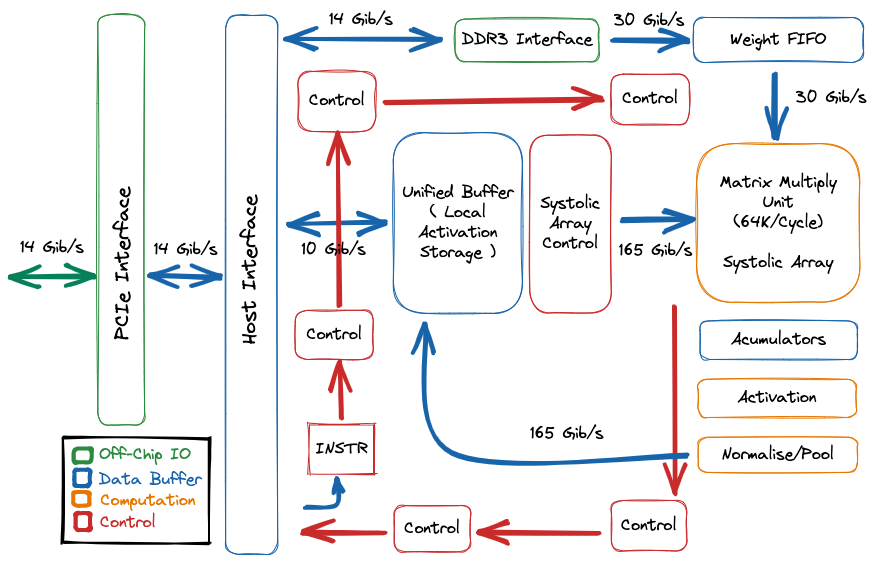
\includegraphics[width=0.65\textwidth]{figures/L1-TPU.png}
    \end{center}
    

    The TPU here is designed to speed up ML and DL. Fast Matrix Multiplication is very
    important to speed up deep learning. So there is a special block for doing that here 
    in the TPU - Systolic Array. Of course we could use an ALU, but it would be extremely slow.
    That is the reason for customisation, we customise the processor to run deep learning
    acceleration. A conventional processor could use the ALU, but it is not effective for 
    matrix multiplications, so customised hardware is necessary to facilitate faster
    processing. 
\end{example}




\section{Key Principles of Custom Computing}
\begin{figure}[H]
    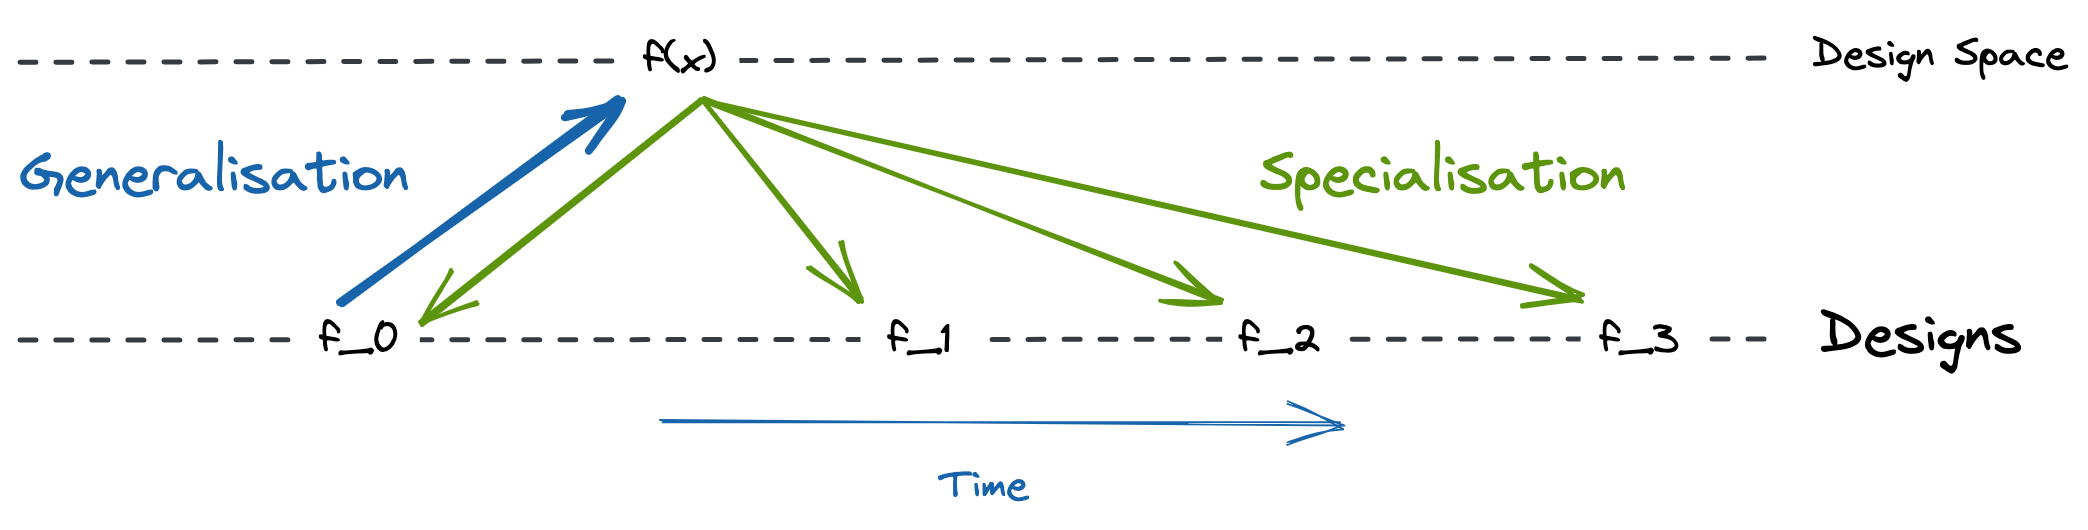
\includegraphics[width=\textwidth]{figures/L1-Generalise+Specialise.png}
    \caption{Principle of Custom Computing}
    \label{fig:generalise-specialise}
\end{figure}

The main principle is to \emph{generalise and specialise} - explained below and 
illustrated in Figure \ref{fig:generalise-specialise}. An experienced designer might 
have a good sleep/dinner and suddenly come up with an optimal solution to a specific problem,
solving for $f_0$. However, this solution for $f_0$ may not be adequate if it needs to 
serve a new application or to exploit new technologies.  This is where \emph{generalisation}
comes in, various methods are tried to generalise $f_0$ to become $f(x)$ where $x$ is a
parameter such than when given the value $x_0$, $f(x)$ \emph{specialises} to $f_0$. 

We say that $f(x)$ forms a design space that can cover for multiple values of $x$. 
One can then select the design that best meets the given requirements in terms of
having the best trade-offs in performance, resource usage, energy consumption etc.
The possibility is that we could also transform the design description to preserve the 
function and provide higher performance. 

\subsection{Benefit of Customisation}
Improvements in:
\begin{itemize}
    \item Accuracy: customisable as needed, could be 2 bits or 128 bits. 
    \item Throughput: rate of results production
    \item Latency: time between first input and first output
    \item Reconfiguration Time: Speed of adapting to change
    \item Size: Area/Volume/Weight
    \item Energy and Power Consumption for mobile applications
    \item Development Time for Design and Verification
    \item Cost: Reduced fabrication time, post-delivery fixes and enhancements all come with FPGAs
\end{itemize}

These all come at a cost, not everything can be achieved, so design objectives 
need to be prioritised. 

\subsection{Implementation Technologies - FPGAs vs ASICs}
\begin{theorem}
    Moore's second law or Rock's law states that the cost of a semiconductor fabrication
    plant doubles every 4 years, increasing exponentially. 

    It is the economic flip side to Moore's first law - that the number of transistors
    in a dense IC double every two years. It is slower, but still exponential. 
    \label{thm:moores-law2}
\end{theorem}

ASICs do support the highest level of customisation as designers can optimise all
the way down to the transistor level in any way, hence providing the greatest efficiency,
at the expense of runtime inflexibility. They are also costly to develop with a high
NRE(non-recurring engineering) cost to ensure efficiency and correctness before going
to silicon production as a chip that does not meet requirements is useless and cannot
be repaired. As Theorem \ref{thm:moores-law2} shows, if the latest technology is used,
the cost of the chip is also very very high!

That's why FPGAs\footnote{An FPGA has memory blocks and arithmetic blocks (coarse-grained) for
fast computation as these are common; and also fine-grained logic blocks for custom computation. } are increasingly popular. They can be used in different applications,
reducing the NRE as the risk is lower with chip behaviour being capable of being changed
at runtime. They have a fast time to market, low development cost and can be customised
at runtime. So what's the catch? Although the initial cost is low, the part cost 
of each FPGA is more expensive than an ASIC. So eventually, there's a break-even point 
where ASICs have better value than FPGAs.  

Recently, FPGAs have become heterogeneous. They have additional processing to do 
special things. See slide 14. This is a double edged sword has these elements 
might not be used for the particular application. But FPGA makers have placed a 
bet on the advancement of ML and hence include these AI engines. 

Another interesting observation is that current civilisation depends the internet.
What enables the internet? One is optical fibre that can carry a lot more data than copper. 
But that is not enough, that data needs to be routed quickly as well to send the packets to 
the correct location. So internet stations use FPGAs to do packet processing to keep up 
with the speed of data transfer. 

Since fabrication becomes more costly, the number of FPGA designs in recent years
has grown a lot faster than ASIC designs.

\begin{figure}
    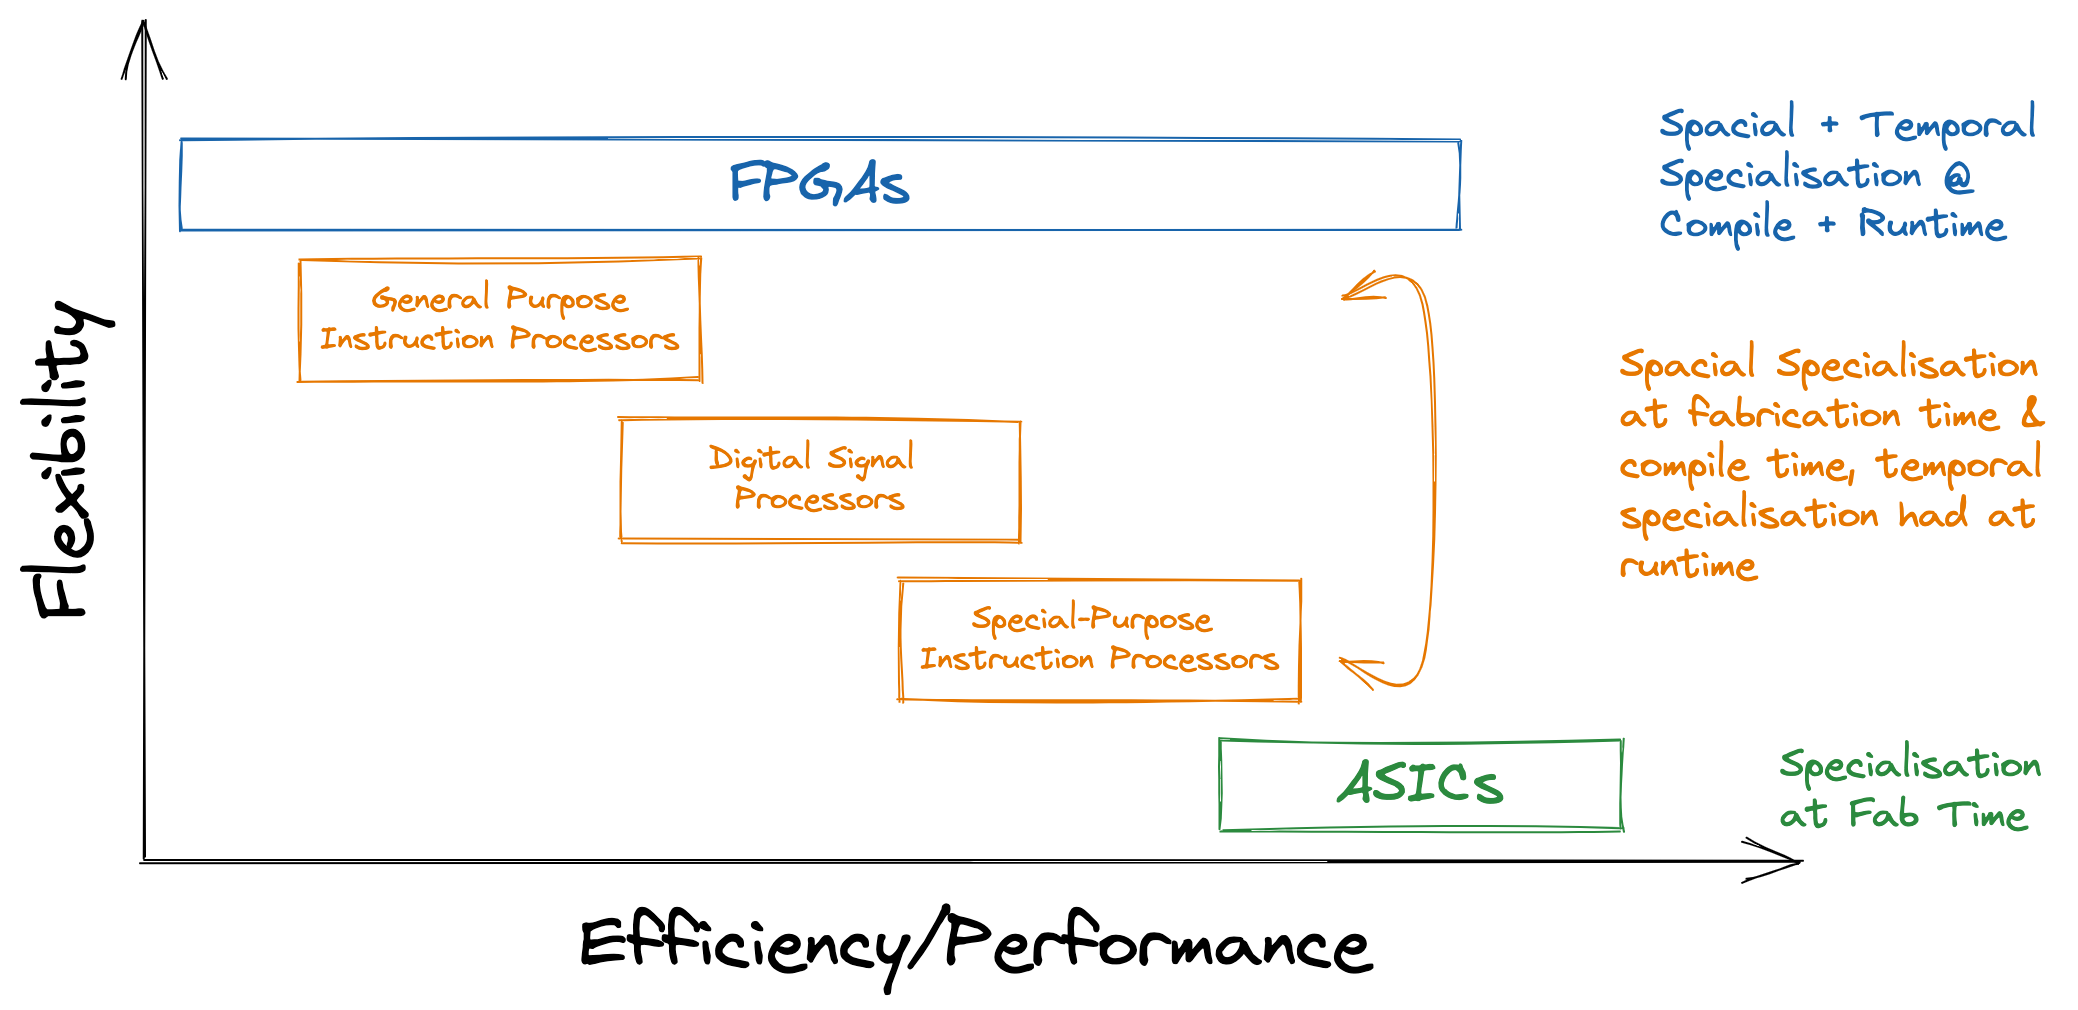
\includegraphics[width=\textwidth]{figures/L1-TechnologyComparison.png}
    \caption{Implementation Technologies Compared}
    \label{fig:fpga-vs-asic}
\end{figure}

\subsubsection{When to Specialise?}

This comparison between ASICs, FPGAs and general purpose computers could also be summarised with this question. 

ASICs would specialise at \emph{fabrication time}. As said, this reduces post-fab options, 
causing reduced flexibility. But the advantage is a lot higher compilation and execution
efficiency. 

FPGAs would mean specialisation at \emph{compilation time}, specialising an initial design
mapping to fabric. This improves execution efficiency at the cost of efficiency for
compilation. Hardware compilation tends to take a long time to compile and execute. 

Or we could specialise at \emph{runtime}. This is the typical instruction processor
that is interpreting instructions at execution. This gives the most flexibility,
but as shown in Table \ref{table:comparison}, the execution efficiency is extremely
low in comparison to ASICs and FPGAs. 


\subsubsection{Makimoto's Wave}
\begin{figure}[H]
    \centering
    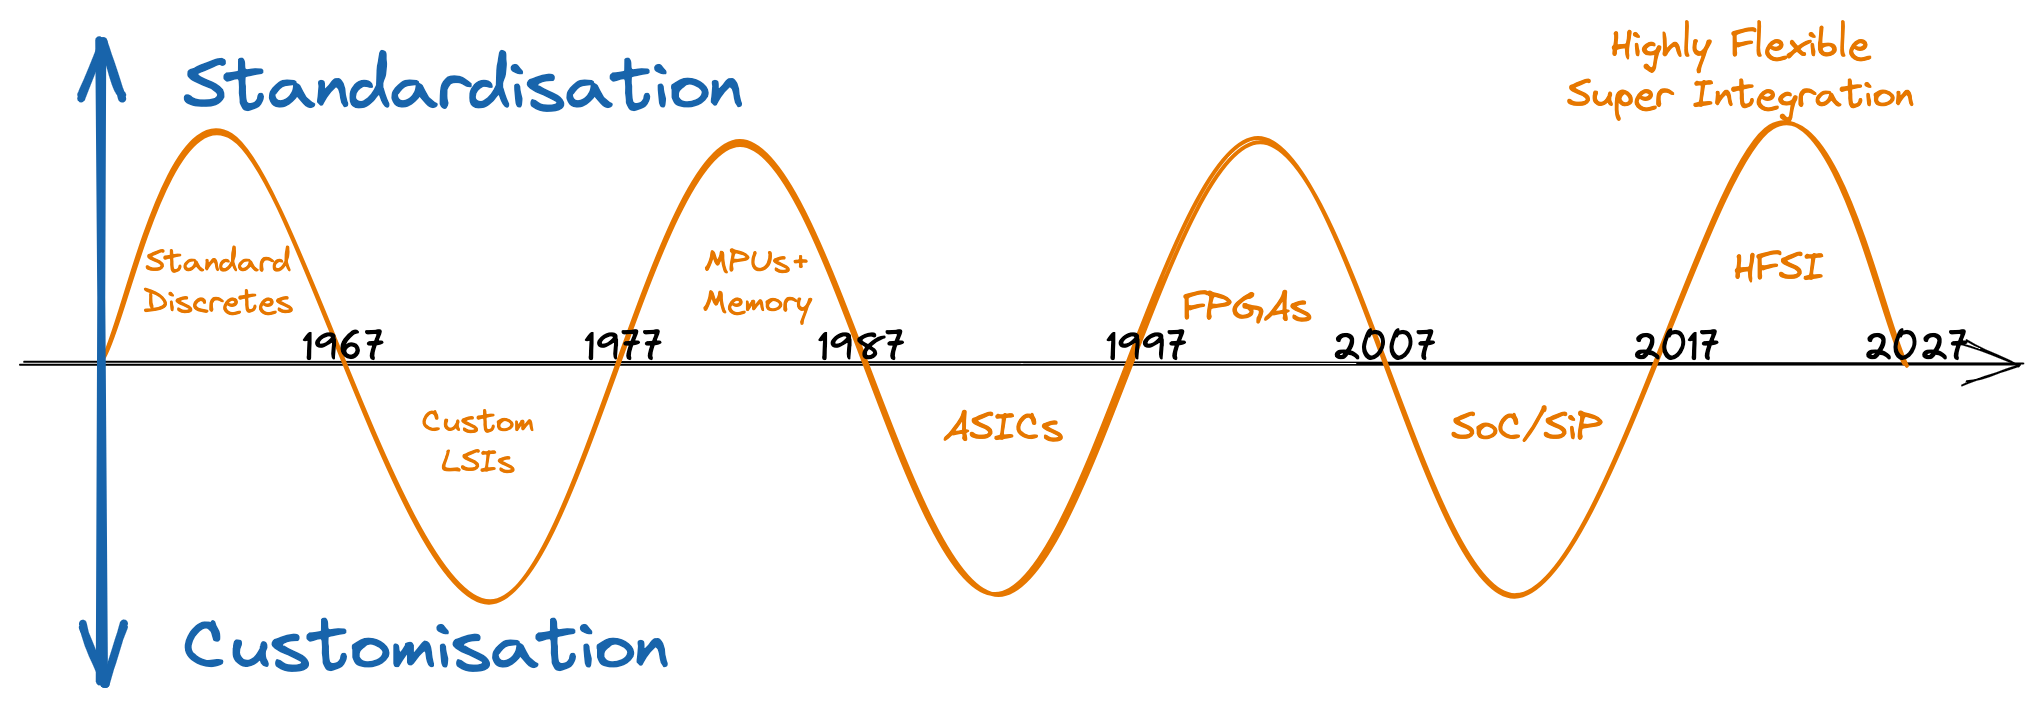
\includegraphics[width=0.8\textwidth]{figures/L1-Makimito.png}
\end{figure}
Makimoto observed that every 10 years there is a change between customisation and standardisation.
It is in part driven by EDA, enabling new types of customisation and the relative costs of each 
solution type.

\subsubsection{Crossover Cost Points between FPGAs and ASICs}
\begin{figure}[H]
    \centering
    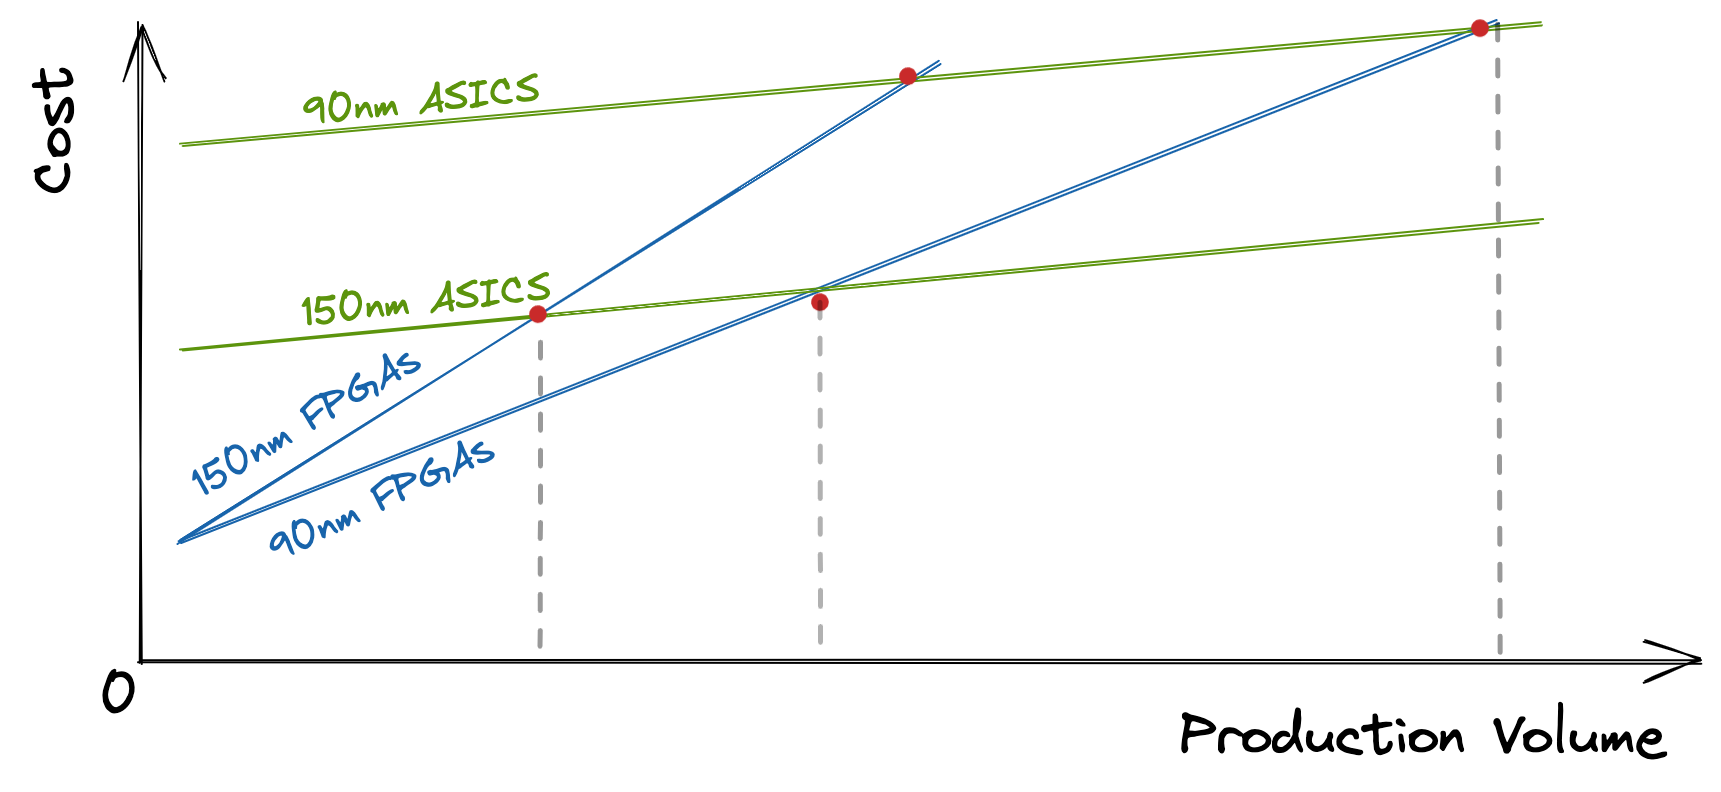
\includegraphics[width=0.8\textwidth]{figures/L1-CrossoverCost.png}
\end{figure}
The slope of the graph represents the replication cost. For ASICs, it is relatively low
because the part cost is lower. As FPGAs have expensive per-part costs, eventually the
overall costs of ASICs at large volumes is lower than the FPGA cost. 

But as technology improves, the effect is different. For the 150nm vs 90nm FPGAs, 
as the technology matures, the cost is reduced. But for ASICS, Moore's second law
applies and has a greater effect thus causing it to become more expensive and moving
the break even point further away. 

\subsubsection{Looking to the future - SoCs}
FPGAs are becoming more heterogeneous as explained earlier. They are
effectively systems-on-a-chip. While fine-grained programmable logic is still
available, the focus will move to how they can interface to coarse-grained
computational and memory resources such as in a system with a hard core and multiple
IP blocks for video processing/machine learning acceleration etc. 
These resources are less flexible but more efficient, and when an application has 
a need for a non-present IP block, it can make use of the integrated programmable
logic to accelerate execution speed. 

\section{Systems and Customisation}
An overview of custom computing systems and how they compare to microprocessors. 

Custom computing systems have been used since 1832 with the first difference engine
by Charles Babbage. From 1993, these custom computing systems began to use FPGAs 
with the Splash2, and this continues to date. 

Custom Computing allows for much higher efficiency. As we move to more computation
happening off device, moving to FPGAs in the cloud would be something that helps 
to reduce the effect of server emissions. 

\subsection{General Purpose vs Special Purpose}

Figure \_ shows an Intel 6-Core X5680. Much of the processor is dedicated to memory. 
General purpose computing requires more chip memory and the computation needs less. 
!! CHECK why does GPC require more memory. 

A chip customised for a specific purpose on the other hand does not require instructions
so no decoder necessary. No need for branch predictions as there are no explicit branches.
There is explicit parallelism, which means no out of order execution. No need for memory
as the data is streamed through the chip. 

\dots

Frequent fetches of instructions from memory cause bottlenecks within the Von 
Neumann architecture - the Von Neumann bottleneck. If a processor can execute 
in a data streaming manner, then the bottleneck is no longer the instruction fetch, 
but how long it actually takes to do the computation. 

\begin{definition}
CPUs are good for control-intensive, non-repetitive code. 

Accelerators are good for kernels with repetitive programs on large data volumes. 

\end{definition}

\begin{example}
    Bing uses FPGAs to accelerate their page ranking service. 
    An example of overcoming performance bottlenecks is provided by
    Microsoft, which shows that their Catapult system with FPGAs can be used in
    enhancing the performance of the Bing search engine, doubling the
    throughput while reducing the latency by almost 30\%. Moreover the number
    of servers are reduced, leading to a cost reduction of 30\%.
\end{example}


\subsection{Programming Custom Computing Systems}

You could do schematic entry, but this becomes a nightmare for large systems. 
Hardware description languages like Verilog and VHDL are good for this, but they 
can also be used as a target language for high level synthesis. 

There are also specific languages at a high level to describe hardware systems. 
This course will cover Ruby (a functional HLS language) and MaxJ (a HLS dataflow language). 

\subsection{The Acceleration Development Flow}

TODO: Insert diagram. 

\subsection{Customisation Techniques}

There are several common opportunities for customisation:
\begin{itemize}
    \item Some data may remain constant - this opens up the opportunity for algebraic simplification
    \item Effective Data Structures - e.g number representation
    \item Data Transformation, either to enhance parallelism or serialisation.
\end{itemize}

There are also several reuse possibilities:
\begin{itemize}
    \item Descriptions
    \item Transforms
\end{itemize}

\subsection{A Customisation Example}

\begin{example}
    If we were to compute:
    \begin{equation}
        y = a_0 + a_1 x + a_2 x^2 +a_3 x^3
    \end{equation}

    This could just be expressed as a for loop and we can have the obvious design. 
\end{example}

\subsubsection{Exploit Algebraic Properties}

We could exploit Horner's Rule:
\begin{equation*}
    ax + bx = (a+b)x
\end{equation*}

And this transformation could be expressed in the following diagrammatic form

\begin{example}
So then our circuit could be transformed to the following:

Reducing the area as the number of multipliers is reduced. 
\end{example}

\subsubsection{Enhance Parallelism}

Reduction can be applied to the circuit. Instead of a sequential addition, 
we can create a balanced tree, reducing the critical path. 

\subsubsection{Pipelining}
Pipelined Verilog Diagram Important Note: Read from Top to Bottom. Input is at the top!



\end{document}
